\documentclass[journal]{IEEEtran}
\usepackage[utf8]{inputenc}

\usepackage[backend=biber]{biblatex}
\usepackage{graphicx}
\usepackage{subcaption}

\addbibresource{references.bib}
 
% - - - - - - - - - - - - - - - - - - - - - - - - - - -

% correct bad hyphenation here
\hyphenation{op-tical net-works semi-conduc-tor}

\begin{document}

\title{Defining and computing entropy for networks}

\author{
Henrique Ferrolho - s1683857,
Team: Alex Hoppen, Charles Desmonty
}

% make the title area
\maketitle

% - - - - - - - - - - - - - - - - - - - - - - - - - - -

\begin{abstract}
\end{abstract}

% - - - - - - - - - - - - - - - - - - - - - - - - - - -

\section{Introduction}

Entropy is the lack of \textit{order} or \textit{predictability}, it is a measure of \textit{randomness} or \textit{disorder} in a system - the greater the disorder the higher the entropy.

We are going to define a measure in order to calculate the entropy of a network graph. But before we do that, we need to agree on what makes a network more or less organized. How does the human notion of order apply to graphs, i.e. having two graphs $A$ and $B$, what properties make graph $A$ more or less organized and structured than graph $B$?

% - - - - - - - - - - - - - - - - - - - - - - - - - - -

\section{Related work}

% - - - - - - - - - - - - - - - - - - - - - - - - - - -

\section{Results}

\begin{figure}[ht]
    \centering
    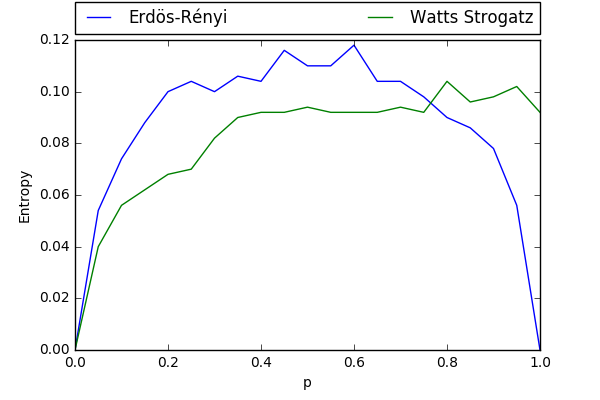
\includegraphics[width=\linewidth]{res/entropy1/experiment_n500.png}
    \caption{TODO.
    }
\end{figure}

\begin{figure}[ht]
    \centering
    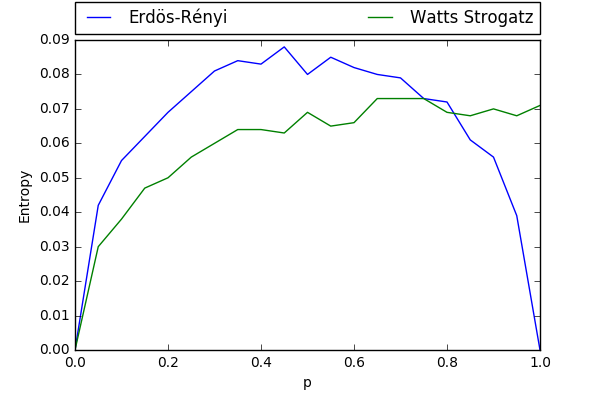
\includegraphics[width=\linewidth]{res/entropy1/experiment_n1000.png}
    \caption{TODO.
    }
\end{figure}

\begin{figure}[ht]
    \centering
    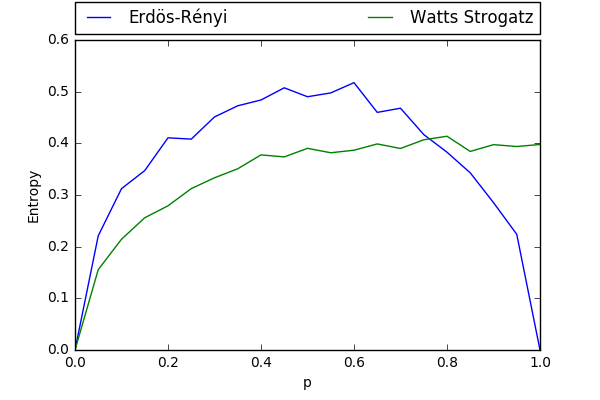
\includegraphics[width=\linewidth]{res/entropy2/experiment_n500.png}
    \caption{TODO.
    }
\end{figure}

\begin{figure}[ht]
    \centering
    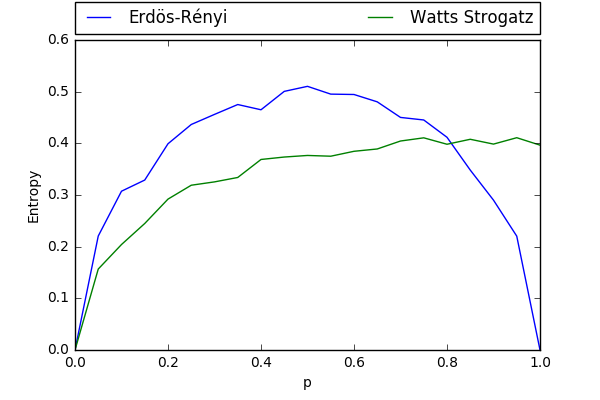
\includegraphics[width=\linewidth]{res/entropy2/experiment_n1000.png}
    \caption{TODO.
    }
\end{figure}

% - - - - - - - - - - - - - - - - - - - - - - - - - - -

\appendices

\section{bla bla bla}

\cite{dehmer2008}
\cite{dehmer2011}
\cite{erdosRenyiGraphs}
\cite{kenley2011}

% - - - - - - - - - - - - - - - - - - - - - - - - - - -

\printbibliography

\end{document}
